\begin{document}
\begin{center}
{\LARGE\bfseries Engineering Higher-Intelligence AI Agents:}\\[6pt]
{\LARGE\bfseries Harness Scaling Across Models and Domains}\\[8pt]
{\large\bfseries A Pre-registered Design for Harness-Scaling, Executor-Comparison\\[2pt]
and Cross-Domain-Transfer Experiments, with the First Measurements}\\[16pt]
{\large Chengshuai Yang$^{1,*}$}\\[5pt]
{\normalsize $^{1}$NextGen PlatformAI C Corp, USA}\\[4pt]
{\normalsize $^{*}$Correspondence: \href{mailto:spiritai@platformai.org}{spiritai@platformai.org}}\\[10pt]
{\small September 3, 2026 --- draft v0.1}
\end{center}

\begin{abstract}
Does harness engineering raise the measured intelligence of an agent, are the gains retained, do they transfer across domains, and does the ranking of base models change under different harnesses? This paper pre-registers the experimental program that answers those questions and reports the measurements that exist so far. The design has three experiments on one benchmark contract: a harness scaling curve that holds the executor fixed and varies the harness generation HG0--HG3; an executor comparison that holds the harness fixed and varies the executor among Claude Code, Codex, OpenCode and Hermes; and a cross-domain transfer test that develops a harness improvement in one of six domains and measures its effect in the other five, summarized by a transfer score $G_i$ with per-domain intervals. Seven hypotheses are stated with their falsifiers, the endpoints are verified completion, false completion, human intervention load and cost per verified completion, and the analysis is a mixed logistic model with executor, harness, domain and executor--harness interaction. The measurements to date cover one domain, three executors from two families, four harness generations instantiated from delegation mechanisms, and one intervention budget. They support harness scaling weakly and executor--harness interaction clearly: two frontier executors moved 3.3 points on a saturated suite while a weaker one moved 15.0, so that the weaker executor was 4.5 times more harnessable and the area-under-curve summary ranked the executors in the opposite order to their gain; the acceptance rung's contribution was exactly zero under the success-only primitive and the whole of the movement under the delivered-outcome primitive, by construction under a paired design; and a fixed solver went from 0/15 to 15/15 under the harness while an executor that could not succeed went from 15/15 wrong-work-delivered to 0/15. Retention held with no task broken by the harness. Human-intervention reduction, self-improvement validity and cross-domain transfer are untested, and the paper says which runs would test them first.
\end{abstract}

\noindent\textbf{Keywords:} harness scaling curve; executor comparison; cross-domain transfer; delegation; false completion; pre-registration; mixed logistic model

\tableofcontents
\bigskip

\section{Introduction}\label{sec:intro}

A base model does not have an intelligence level; a frozen model--harness pair does \citep{yang2026unified}. That statement has an engineering corollary and an experimental obligation. The corollary is that the way to a higher measured level is to build the harness, and \citet{yang2026agents} gives the design method. The obligation is to show, on a frozen benchmark that the harness cannot edit, that harness engineering actually moves the measurement --- and to show it in a way that separates the harness effect from the executor effect, the domain effect, and their interaction.

This paper is the pre-registration of that program and the report of its first measurements. It is written before the program has run in full, on purpose: the hypotheses, endpoints, model and falsifiers are stated here so that later results are read against them rather than fitted to them. What has run is one domain, three executors, four harness generations and one intervention budget. What has not run is stated in \S\ref{sec:coverage} in the order it should.

\subsection{Contributions}

\begin{enumerate}[leftmargin=*]
\item \textbf{Seven hypotheses with falsifiers} (\S\ref{sec:hypotheses}), from harness scaling to benchmark centrality.
\item \textbf{Three experiments on one contract} (\S\ref{sec:design}): the harness scaling curve, the executor comparison, and the cross-domain transfer test, with the distinction between the first two made explicit because it is the one most often elided.
\item \textbf{Endpoints, statistical model and matched designs} (\S\ref{sec:stats}).
\item \textbf{First measurements} (\S\ref{sec:results}): three harness scaling curves, two paired rung comparisons, an arms study, and one executor comparison, read against the hypotheses.
\item \textbf{Coverage of the pre-registered matrix} (\S\ref{sec:coverage}) and the next runs in cost order.
\end{enumerate}

\section{Hypotheses and Falsifiers}\label{sec:hypotheses}

\begin{table}[H]
\centering\small
\begin{tabularx}{\textwidth}{@{}lYY@{}}
\toprule
& Hypothesis & Falsified if \\
\midrule
H1 & Harness scaling: $P(\text{verified completion} \mid HG_{n+1}) > P(\cdot \mid HG_n)$ under matched executor, task, resources and budget & harness generations do not improve frozen benchmark scores, or improve headline scores while increasing false completion \\
H2 & Intervention reduction: higher generations reduce required $H$ at fixed $T$ and reliability & human intervention remains high across generations \\
H3 & Retention: new capability does not materially degrade lower-level certified capability & higher-level mechanisms cause lower-level regressions \\
H4 & Cross-domain transfer: some harness improvements developed in one domain improve unrelated domains & every improvement is domain-specific \\
H5 & Self-improvement validity: HG3 candidates outperform the frozen baseline on hidden evaluations more often than matched non-adaptive controls & agent-designed improvements work only when the agent can influence the evaluator \\
H6 & Executor--harness interaction: the strongest base executor is not necessarily the strongest agent under every harness & executor ranking is invariant to harness \\
H7 & Benchmark centrality: architectures that look more sophisticated do not earn higher levels unless frozen benchmark performance improves & --- (a methodological commitment rather than a falsifiable claim) \\
\bottomrule
\end{tabularx}
\caption{The seven hypotheses of \citet{yang2026plan} \S31 with the falsifiers of \S30. A falsification is a useful outcome, not a failed publication.}
\label{tab:hyp}
\end{table}

Two further falsifiers apply to the program as a whole: the same effects disappear under hidden tasks, or benchmark items cannot be validated reliably. Both are addressed by the benchmark contract rather than by the experiments \citep{yang2026uab}.

\section{Design}\label{sec:design}

\subsection{The benchmark contract}

All three experiments run on the Unified Agent Benchmark contract \citep{yang2026uab}: a frozen pair, the delivered-outcome primitive $S^{\text{net}}_A = P(\text{delivered and verifier pass}) - \rho\,P(\text{false completion})$, four derived outcomes, an episode record that carries why the episode ended, an acceptance locus that is never the performing system, and a hard gate with retention. Nothing below is interpretable without it.

\subsection{Experiment B: the harness scaling curve}

Hold the executor fixed. Vary the harness generation. For frozen $m$ and generation $HG_k$, $HSC_m(k) = HLIS(m, HG_k)$; the ordered set is the curve, and the curve is the primary result. Summaries --- HIL-Level, HIL-AUC, HIL-Ceiling, Harness Gain --- are conveniences and one of them is shown below to mislead.

Each rung is a strict superset of the one below, enforced by a test, because otherwise a difference between rungs is attributable to nothing. Two rungs that differ only in post-hoc machinery (HG0 versus HG1) are scored from the same executor outputs, because independent runs introduce between-rung variance that exceeds the effect.

\subsection{Experiment A: the executor comparison}

Hold the harness fixed. Vary the executor: Claude Code, Codex, OpenCode, Hermes, and a local model where available, behind one executor protocol so the harness never learns which vendor it is talking to. Same benchmark, tasks, tools, resources, budget and verifier. Tool authority is equalised or recorded as unequal.

\begin{cautionbox}{A is not B}
Changing the executor at fixed harness asks a different question from changing the harness at fixed executor. A matched executor comparison is not a harness scaling curve segment, and reporting it as one is the elision this design is written to prevent. The regime-switch result in \S\ref{sec:results} is an Experiment A instance and is labelled so.
\end{cautionbox}

\subsection{Experiment C: cross-domain transfer}

Develop a harness improvement $i$ in one domain. Test it, unchanged, in the other five. Define $\Delta_{i,d} = P_{i,d} - P_{\text{baseline},d}$ and
\[
G_i = \frac{1}{|D|}\sum_{d \in D} \Delta_{i,d},
\]
with per-domain confidence intervals reported beside the mean. An improvement that moves one domain is domain engineering; one that moves several unrelated domains is evidence of a general mechanism. Candidate mechanisms, each testable as a single change: memory, failure classification, rollback, evidence verification, planner, routing, self-model, learning procedure.

\subsection{Endpoints}

Primary: verified completion, false completion, human-intervention count and depth, cost per verified completion. Secondary: false rejection, held-back rate, wall time, tokens, retry count, regression count, restart success (U1), learning transfer (U2), self-improvement gain (U3). Every result carries the resource envelope; equal scores at unequal cost are unequal results.

\section{Statistical Structure}\label{sec:stats}

For task $i$, executor $m$, harness $h$ and domain $d$, let $Y_{imhd} \in \{0,1\}$ be verified completion. The pre-registered model is
\[
\operatorname{logit} P(Y_{imhd} = 1) = \beta_0 + \beta_m + \beta_h + \beta_d + \beta_{mh} + u_i,
\]
with a random task effect $u_i$. The executor--harness interaction $\beta_{mh}$ is the term H6 lives in. False completion is modelled the same way as a second outcome, never folded into the first. Matched designs are used wherever the comparison permits: the same seeds across executors, the same executor outputs across post-hoc rungs, the same task family across budgets.

Sample sizes in the archived runs are readings, not rates: twelve episodes per rung, two seeds per class. The pre-registered minimum for a rate is four seeds per class per cell, with Clopper--Pearson intervals reported per band and every frontier $F_A(H,p)$ labelled provisional below that.

\section{Apparatus}\label{sec:apparatus}

The reference ladder \texttt{dli-ladder/HG0--HG3} instantiates the first four generations from delegation-harness mechanisms: HG0 the executor, bounded tools and an evidence log with no acceptance step; HG1 persistent state, a criterion registered before the work and acceptance in a separate process; HG2 snapshot, restore and retry with the failed check named; HG3 failure classification, a competence model and routing across executors. HG0 has no acceptance step on purpose: it is the configuration a contemporary leaderboard measures, and its false-completion rate is the number every higher rung is measured against.

\begin{cautionbox}{Naming: the built HG3 is not the plan's HG3}
The development plan names HG3 the self-improving generation, with governed candidate modification of prompts, policies and routing under a frozen hidden evaluation. The built ladder's HG3 is the delegation instantiation --- classification and routing --- and contains no self-modification. Every result below is therefore about delegation mechanisms at HG0--HG3, and H5 is untested by them.
\end{cautionbox}

Before any episode: the pair is frozen (model identity from a live call, harness manifest hash, tool grant, memory snapshot, host, enforced timeout), and seven apparatus checks run as positive controls. Three apparatus bugs in this program's history each produced a plausible wrong result invisible from the code: derived checks passed through an interpreter with escaped newlines and never executed, so a first run scored 15/15 and was meaningless; a timeout that killed only the direct child while its children held the pipe, so a killed run was scored as delivered nothing; and a limit that fired correctly but was shorter than the task. Every episode now records why it ended.

\section{First Measurements}\label{sec:results}

All measurements below are in one domain (software and data tasks), on six task classes at T0--T3 with two seeds each, at H1, on the reference ladder. Three executors from two vendor families were run: Claude Code with its default model, Codex, and Claude Code with a weaker model. Absolute values are not claims about any product.

\subsection{Three harness scaling curves}

\begin{table}[H]
\centering\small
\begin{tabularx}{\textwidth}{@{}lYcccccc@{}}
\toprule
Executor & Rung & $A_{DI}^{\text{raw}}$ & $HLIS_{DI}$ & net ($\rho{=}1$) & false-done & held back & attempts \\
\midrule
Family A, stronger & HG0 & 0.933 & 93.3 & 86.7 & 2 & 0 & 12 \\
 & HG1 & 0.933 & 93.3 & 93.3 & 0 & 2 & 12 \\
 & HG2 & 0.967 & 96.7 & 96.7 & 0 & 1 & 15 \\
 & HG3 & 0.967 & 96.7 & 96.7 & 0 & 1 & 14 \\
\midrule
Family B & HG0 & 0.933 & 93.3 & 86.7 & 2 & 0 & 12 \\
 & HG1 & 0.933 & 93.3 & 93.3 & 0 & 2 & 12 \\
 & HG2 & 0.967 & 96.7 & 96.7 & 0 & 1 & 16 \\
 & HG3 & 0.967 & 96.7 & 96.7 & 0 & 1 & 15 \\
\midrule
Family A, weaker & HG0 & 0.783 & 78.3 & 56.7 & 4 & 0 & 12 \\
 & HG1 & 0.917 & 91.7 & 91.7 & 0 & 3 & 12 \\
 & HG2 & 0.917 & 91.7 & 91.7 & 0 & 3 & 18 \\
 & HG3 & 0.933 & 93.3 & 93.3 & 0 & 2 & 14 \\
\bottomrule
\end{tabularx}
\caption{Three harness scaling curves on \texttt{dli-ladder/HG0--HG3}, 48 episodes per executor, all at H1, band weights 1, 2, 4, 8. Families A and B are two vendor CLIs.}
\label{tab:hsc}
\end{table}

\begin{figure}[H]
\centering
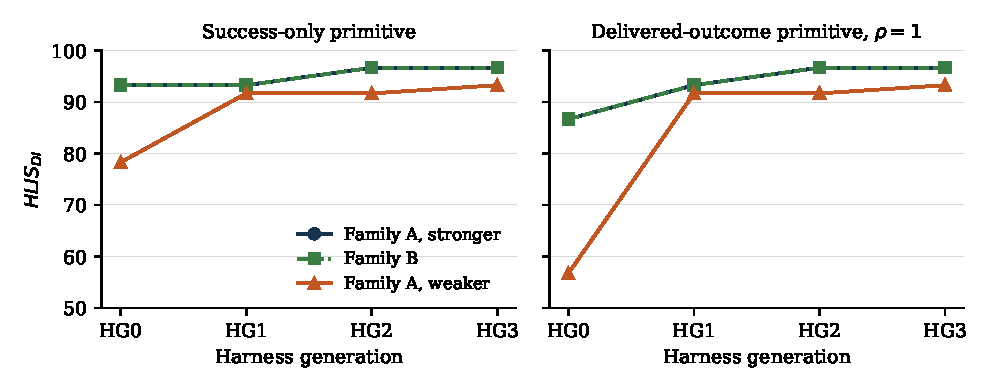
\includegraphics[width=\textwidth]{fig_hsc.pdf}
\caption{The three curves under the success-only primitive (left) and the delivered-outcome primitive at $\rho=1$ (right). The two frontier executors coincide on both panels.}
\label{fig:hsc}
\end{figure}

\begin{table}[H]
\centering\small
\begin{tabularx}{\textwidth}{@{}lcccY@{}}
\toprule
& A stronger & B & A weaker & Reading \\
\midrule
$HLIS_{DI}(HG0)$ & 93.3 & 93.3 & 78.3 & the weaker executor starts far behind \\
HIL-Ceiling & 96.7 & 96.7 & 93.3 & and ends behind \\
Harness Gain (gross) & 3.3 & 3.3 & 15.0 & but is 4.5$\times$ more harnessable \\
Harness Gain (net) & 10.0 & 10.0 & 36.6 & the acceptance rung is the largest step \\
HIL-AUC & 95.0 & 95.0 & 88.8 & ranks by baseline, not by harness response \\
\bottomrule
\end{tabularx}
\caption{Curve summaries. HIL-AUC ranks the executors in the opposite order to Harness Gain, which is why the curve is primary and the composite a convenience.}
\label{tab:summary}
\end{table}

\textbf{Against H1.} Supported weakly and with a qualification. Every executor's curve is non-decreasing and every one moves between HG0 and HG2. But the two frontier executors moved 3.3 gross points on a suite where they had 6.7 points of headroom, and they produced the same aggregate curve to three significant figures while failing different seeds at different cost (53 versus 55 attempts, a factor of two to three in wall clock). Two independent systems agreeing to three figures while differing in which instances they fail is the signature of a saturated suite, not of equivalent systems. The frontier segment of H1 is therefore unresolved by this suite; the weaker executor's 15.0-point gain is the H1 evidence.

\textbf{Against H6.} Supported. The area-under-curve summary orders the executors by baseline, and the gain orders them the other way. Which executor is ``strongest'' depends on which harness it is read at, which is what H6 asserts.

\textbf{Against H3.} Held. Across the frontier executors' 20 bare-versus-harnessed episodes, zero tasks were broken by the harness and two were turned around by it; no lower band regressed at any rung.

\textbf{Against H2.} One reading, from the budget-cross runs of the benchmark paper \citep{yang2026uab}: on six T0/T1 families at three budgets, the executor never used the H1 clarification, and the one H2 local correction it received turned a false completion into a delivered-correct outcome. Intervention reduces false completion on that episode; nothing is established about required $H$ at fixed reliability, because the suite is saturated at H0 on every band present.

\subsection{The paired rung comparison}

\begin{table}[H]
\centering\small
\begin{tabularx}{\textwidth}{@{}lcccYc@{}}
\toprule
Executor & Gross HG0 & Gross HG1 & Difference & Net HG0 $\to$ HG1 & False rejections \\
\midrule
A, stronger & 0.933 & 0.933 & 0.000000 & $0.867 \to 0.933$ ($+0.067$) & 0 \\
A, weaker & 0.917 & 0.917 & 0.000000 & $0.833 \to 0.917$ ($+0.083$) & 0 \\
\bottomrule
\end{tabularx}
\caption{HG0 and HG1 scored from the same executor outputs, twelve episodes per executor. The gross difference is zero by construction; the entire contribution of the acceptance rung appears in the net figure.}
\label{tab:paired}
\end{table}

The weaker executor's earlier independent-run curve showed HG0 $\to$ HG1 rising from 78.3 to 91.7; under pairing that rise is zero on the gross primitive, so it was between-run noise larger than the effect. This is the design consequence stated in \S\ref{sec:design}: any pair of rungs that do not differ in what the executor is asked to do are scored from one execution. Zero false rejections across all 24 paired episodes is what makes the net primitive safe to adopt here: the acceptance step declined exactly the work the external verifier rejected and nothing else.

\subsection{The arms study}

\begin{table}[H]
\centering\small
\begin{tabularx}{\textwidth}{@{}lYl@{}}
\toprule
Arm & Configuration & Result \\
\midrule
1 & capable but careless solver, bare & 0/15 passed \\
2 & the same solver, harnessed & 15/15 passed \\
3 & an executor that cannot succeed, bare & 15/15 wrong work returned as done \\
3$'$ & the same executor, harnessed & 0/15 wrong work returned; 15/15 escalated \\
4 & routed over both, learning from verdicts & 15/15 passed \\
\bottomrule
\end{tabularx}
\caption{Five task classes, three seeds, one solver family, four arms. Nothing about the solver differs between arms.}
\label{tab:arms}
\end{table}

Arm 3 is the one that matters for H1's qualification about false completion: a retry loop runs a hopeless executor three times and returns the third wrong answer; a delegation harness must never report it as done, and did not. Arm 4's router started with no evidence, watched the independent verifier reject the stubborn executor, classified the second failure as capability rather than bad luck, and moved the work; its competence table is built only from independent verdicts, and an executor's own account of how it went never enters it.

\subsection{An executor comparison at fixed harness}

On the sealed regime-switch family, with harness, protocol, timeout and twelve common seeds held fixed, the frontier executor passed 5/12 and a weaker one 1/12; four pairs were discordant, all in the frontier's favour, with an exact two-sided McNemar $p = 0.125$; the frontier's RMSE was lower on 11/12 pairs, with an exact sign test $p = 0.00635$ \citep{yang2026unified}. This is an Experiment A instance: it discriminates the archived configurations on these instances, it is not a curve segment, and the frontier executor's identity is missing from the archived record --- a freeze omission the apparatus rules now prevent.

\subsection{A matched executor comparison on every domain}\label{sec:execcmp}

The six in-package T0/T1 families of the benchmark \citep{yang2026uab} were run on identical seeds at H0, H1 and H2 --- 72 episodes per pair --- by three pairs. Two are a true executor swap at fixed harness: Claude Code 2.1.258 with its default model, and the same Claude Code with Qwen 3.8 (27B) behind it, reached through a local proxy that rewrites the model name and hoists system messages for the serving shim. The third is a different pair, not an executor swap: OpenCode 1.18.27 with the free Muse Spark 1.3 model, so its harness differs as well and it is reported as a pair rather than as a row of Experiment A.

\begin{table}[H]
\centering\small
\begin{tabularx}{\textwidth}{@{}lcccccclccY@{}}
\toprule
& \multicolumn{3}{c}{T0 (20 per budget)} & \multicolumn{3}{c}{T1 (4 per budget)} & & & & \\
Pair & H0 & H1 & H2 & H0 & H1 & H2 & Total & FC & Mean s & Note \\
\midrule
Claude Code, default model & 20 & 20 & 20 & 4 & 4 & 4 & 72/72 & 0 & 28.6 & after one item repair (\S\ref{sec:results}) \\
Claude Code, Qwen 3.8 (27B) & 20 & 20 & 20 & 4 & 4 & 4 & 72/72 & 0 & 90.6 & same harness; executor swapped \\
OpenCode, Muse Spark 1.3 & 20 & 20 & 19 & 4 & 4 & 4 & 71/72 & 1 & 22.5 & different harness; a third pair \\
\bottomrule
\end{tabularx}
\caption{Matched comparison on the six T0/T1 families, four seeds, three budgets. No pair asked a clarifying question in any of its 48 opportunities, so by the zero-intervention rule every H1 episode and all but one H2 episode are H0 episodes. FC is false completions. Records are released with the benchmark.}
\label{tab:execcmp}
\end{table}

\textbf{Reading.} The suite is saturated for all three pairs: 215 of 216 episodes pass, and the one failure is an OpenCode episode at H2 on a seed the same pair passed at H0 and H1, where the executor reported done twice without changing the file. Per-band headroom is zero for every pair, so this comparison discriminates nothing about capability and says something definite about cost: at equal scores the Qwen pair took three times the wall clock of the default pair and four times that of the OpenCode pair, which is the ``equal scores, unequal costs'' result of \S\ref{sec:results} again, on a second suite and an open model. It also answers a narrower question the design asked: the harness effect is not a property of one vendor's model, since the same harness carried an open 27B model to the same surface.

\textbf{Against H6 and H7.} Nothing here can reorder executors, because nothing here separates them; the reordering evidence remains the ladder curves. The comparison is instead the clearest instance yet of H7: three pairs of visibly different sophistication earn the same reading on a frozen suite, and the difference among them is invisible until an item has headroom. The next executor comparison should be run on the sealed families, not on these.

\textbf{Apparatus, again.} Two defects were found and fixed before these numbers were produced: OpenCode resolves its working directory from an environment variable the runner had not set, so its first run did every episode's work in the runner's own directory and failed all of them; and the Qwen shim rejects system-role messages that are not first, which Claude Code 2.1.258 emits, so the proxy hoists them. Both would have read as executor failures.

\subsection{What these measurements do not show}

Any cross-domain transfer (H4): one domain. Any intervention reduction (H2): one budget. Any self-improvement validity (H5): no self-modifying rung was built. Any model-tier ordering: two vendor families on the ladder, one host, one operator; the three-pair comparison of \S\ref{sec:execcmp} separates nothing because its suite is saturated. Any rate: twelve episodes per rung are readings.

\section{Coverage of the Pre-registered Matrix}\label{sec:coverage}

\begin{table}[H]
\centering\small
\begin{tabularx}{\textwidth}{@{}lYY@{}}
\toprule
Factor & Pre-registered & Measured to date \\
\midrule
Executors & Claude Code, Codex, OpenCode, Hermes, local & Claude Code (two models), Codex on the ladder; Claude Code with Qwen 3.8 and OpenCode with Muse Spark 1.3 on the T0/T1 families; Hermes adapter only \\
Harness generations & HG0--HG3 as specified, then HG4--HG5 & HG0--HG3 as the delegation instantiation; no self-modifying rung \\
Domains & paper, funding, job, code, research, business & code (six classes); one sealed research family; the six in-package T0/T1 families run by three pairs at three budgets (saturated); the U2 learning-transfer suite bound and run on two seeds with one pair (transfer on both, ablated arm fails); the U3 suite run once (promoted) \\
Intervention budgets & H0, H1, H2 standardized & H1 only on the ladder; H0/H1/H2 on the six in-package T0/T1 families (72 episodes, one pair): no question asked in 48 opportunities, one H2 correction turned a false completion into a pass \\
Seeds per class & $\ge 4$ & 2 (ladder), 3 (arms), 1 (regime switch) \\
Transfer test & six domains, $G_i$ with intervals & none \\
\bottomrule
\end{tabularx}
\caption{What has run against what was pre-registered.}
\label{tab:coverage}
\end{table}

The next runs, in the order that costs least and unblocks most: the bound code families at H0 and H2, so the frontier profile is computable and H2 has its first reading; four seeds per class on the same families, so readings become rates; OpenCode on the same ladder, so the harness effect is shown on an open executor; the five new T0/T1 families, now bound and live-checked, on the same ladder, so every domain enters the transfer test at its lowest band; and a self-modifying HG3 with a sandbox, frozen hidden evaluation and independent promoter, so H5 has a test at all.

\section{Limitations}\label{sec:limits}

\begin{itemize}[leftmargin=*]
\item \textbf{The suite is saturated for frontier executors}, so the frontier segment of H1 is unresolved by it. Harder items desaturate it only outside the mechanically-derivable envelope; the sealed regime-switch family is the first such and has one mechanism family.
\item \textbf{One domain, one budget, two vendor families, one host.} Every generalization in \S\ref{sec:results} is bounded by those four facts.
\item \textbf{The built ladder is the delegation instantiation.} HG3 here contains no self-modification; H5 is untested.
\item \textbf{The arms study uses reference solvers}, not live executors, for arms 1 to 4; it establishes that the harness moved the outcome, not a rate for any product.
\item \textbf{Readings, not rates.} Twelve episodes per rung; the difference between 0.933 and 0.967 is one episode.
\item \textbf{One archived executor is unnamed.} The regime-switch frontier run has no model identity in its record.
\end{itemize}

\section{Conclusion}

The program asks whether harness engineering raises measured intelligence, whether the gains hold, whether they transfer, and whether the ranking of base models depends on the harness they are read at. The design separates those questions into three experiments on one contract and states seven hypotheses with the observations that would falsify them. The measurements so far answer the last question most clearly --- the composite summary and the harness gain rank the same executors in opposite orders --- and answer the first with a qualification the suite forces: the frontier executors had almost no headroom, and the weaker executor's gain of fifteen points is the harness-scaling evidence. The acceptance rung's contribution was zero under the success-only primitive and the whole of the movement under the delivered-outcome one, exactly as the primitive predicts, and a fixed solver went from nothing to everything under the harness while an executor that could not succeed stopped delivering wrong work as done. Retention held. Transfer, intervention reduction and self-improvement are untested, and the runs that would test them are listed in the order they should be run. That list, not the numbers, is the paper's main result.

\section*{Availability}

The ladder, arms and paired results are archived in \url{https://github.com/integritynoble/AI4Science} under \texttt{ai4science/harness/agents/delegation/} and in the v2.0 paper dataset of \url{https://github.com/integritynoble/sarsi-intelligence-level}. The benchmark contract is in the same corpus under \texttt{uab\_v01/}.

\section*{Conflicts and funding}

The author reports no funding specific to this work and no competing interest.
